\section{问题一:两组专家对同批教师教学评价的差异性与可信度分析}


\subsection{建模思路与分析流程}
本节思路如下:

\begin{enumerate}
    \item \textbf{数据预处理与批量求和}:针对原始多层次评分表,对每位教师、每组专家的11项具体指标分数求和,得出教师—专家—组的总分数据。对于极个别缺失情况,采用“同一教师该指标其他专家均值补齐”策略,确保数据完整性。
    \item \textbf{描述性统计分析}:对两组专家评分总分计算均值、中位数、标准差、极差、偏度、峰度等,并通过箱线图、直方图展示分布,为后续检验提供支持。
    \item \textbf{显著性差异检验与效应量分析}:考虑到数据为同一批教师的配对评分,首先进行差值的正态性检验(Shapiro-Wilk),如通过则用配对t检验,否则用Wilcoxon符号秩检验。进而计算Cohen's $d$,定量衡量实际意义。
    \item \textbf{内部一致性与可信度评价}:采用组内相关系数ICC(双向随机效应、绝对一致性、单次测量模型 ICC(2,1)),分析每组专家评分的一致性,值越大可信度越高。
    \item \textbf{综合判据与结论}:整合差异显著性、效应大小与ICC,系统比较两组专家数据的可靠性。
\end{enumerate}

\subsection{数据处理与描述性统计}


\begin{itemize}
    \item $n$:参评教师人数。
    \item $S^{(1)}_i$:第$i$位教师第一组专家的平均总分。
    \item $S^{(2)}_i$:第$i$位教师第二组专家的平均总分。
    \item $D_i = S^{(1)}_i - S^{(2)}_i$:第$i$位教师两组评分平均值差异。
\end{itemize}

\begin{figure}[htbp]
    \centering
    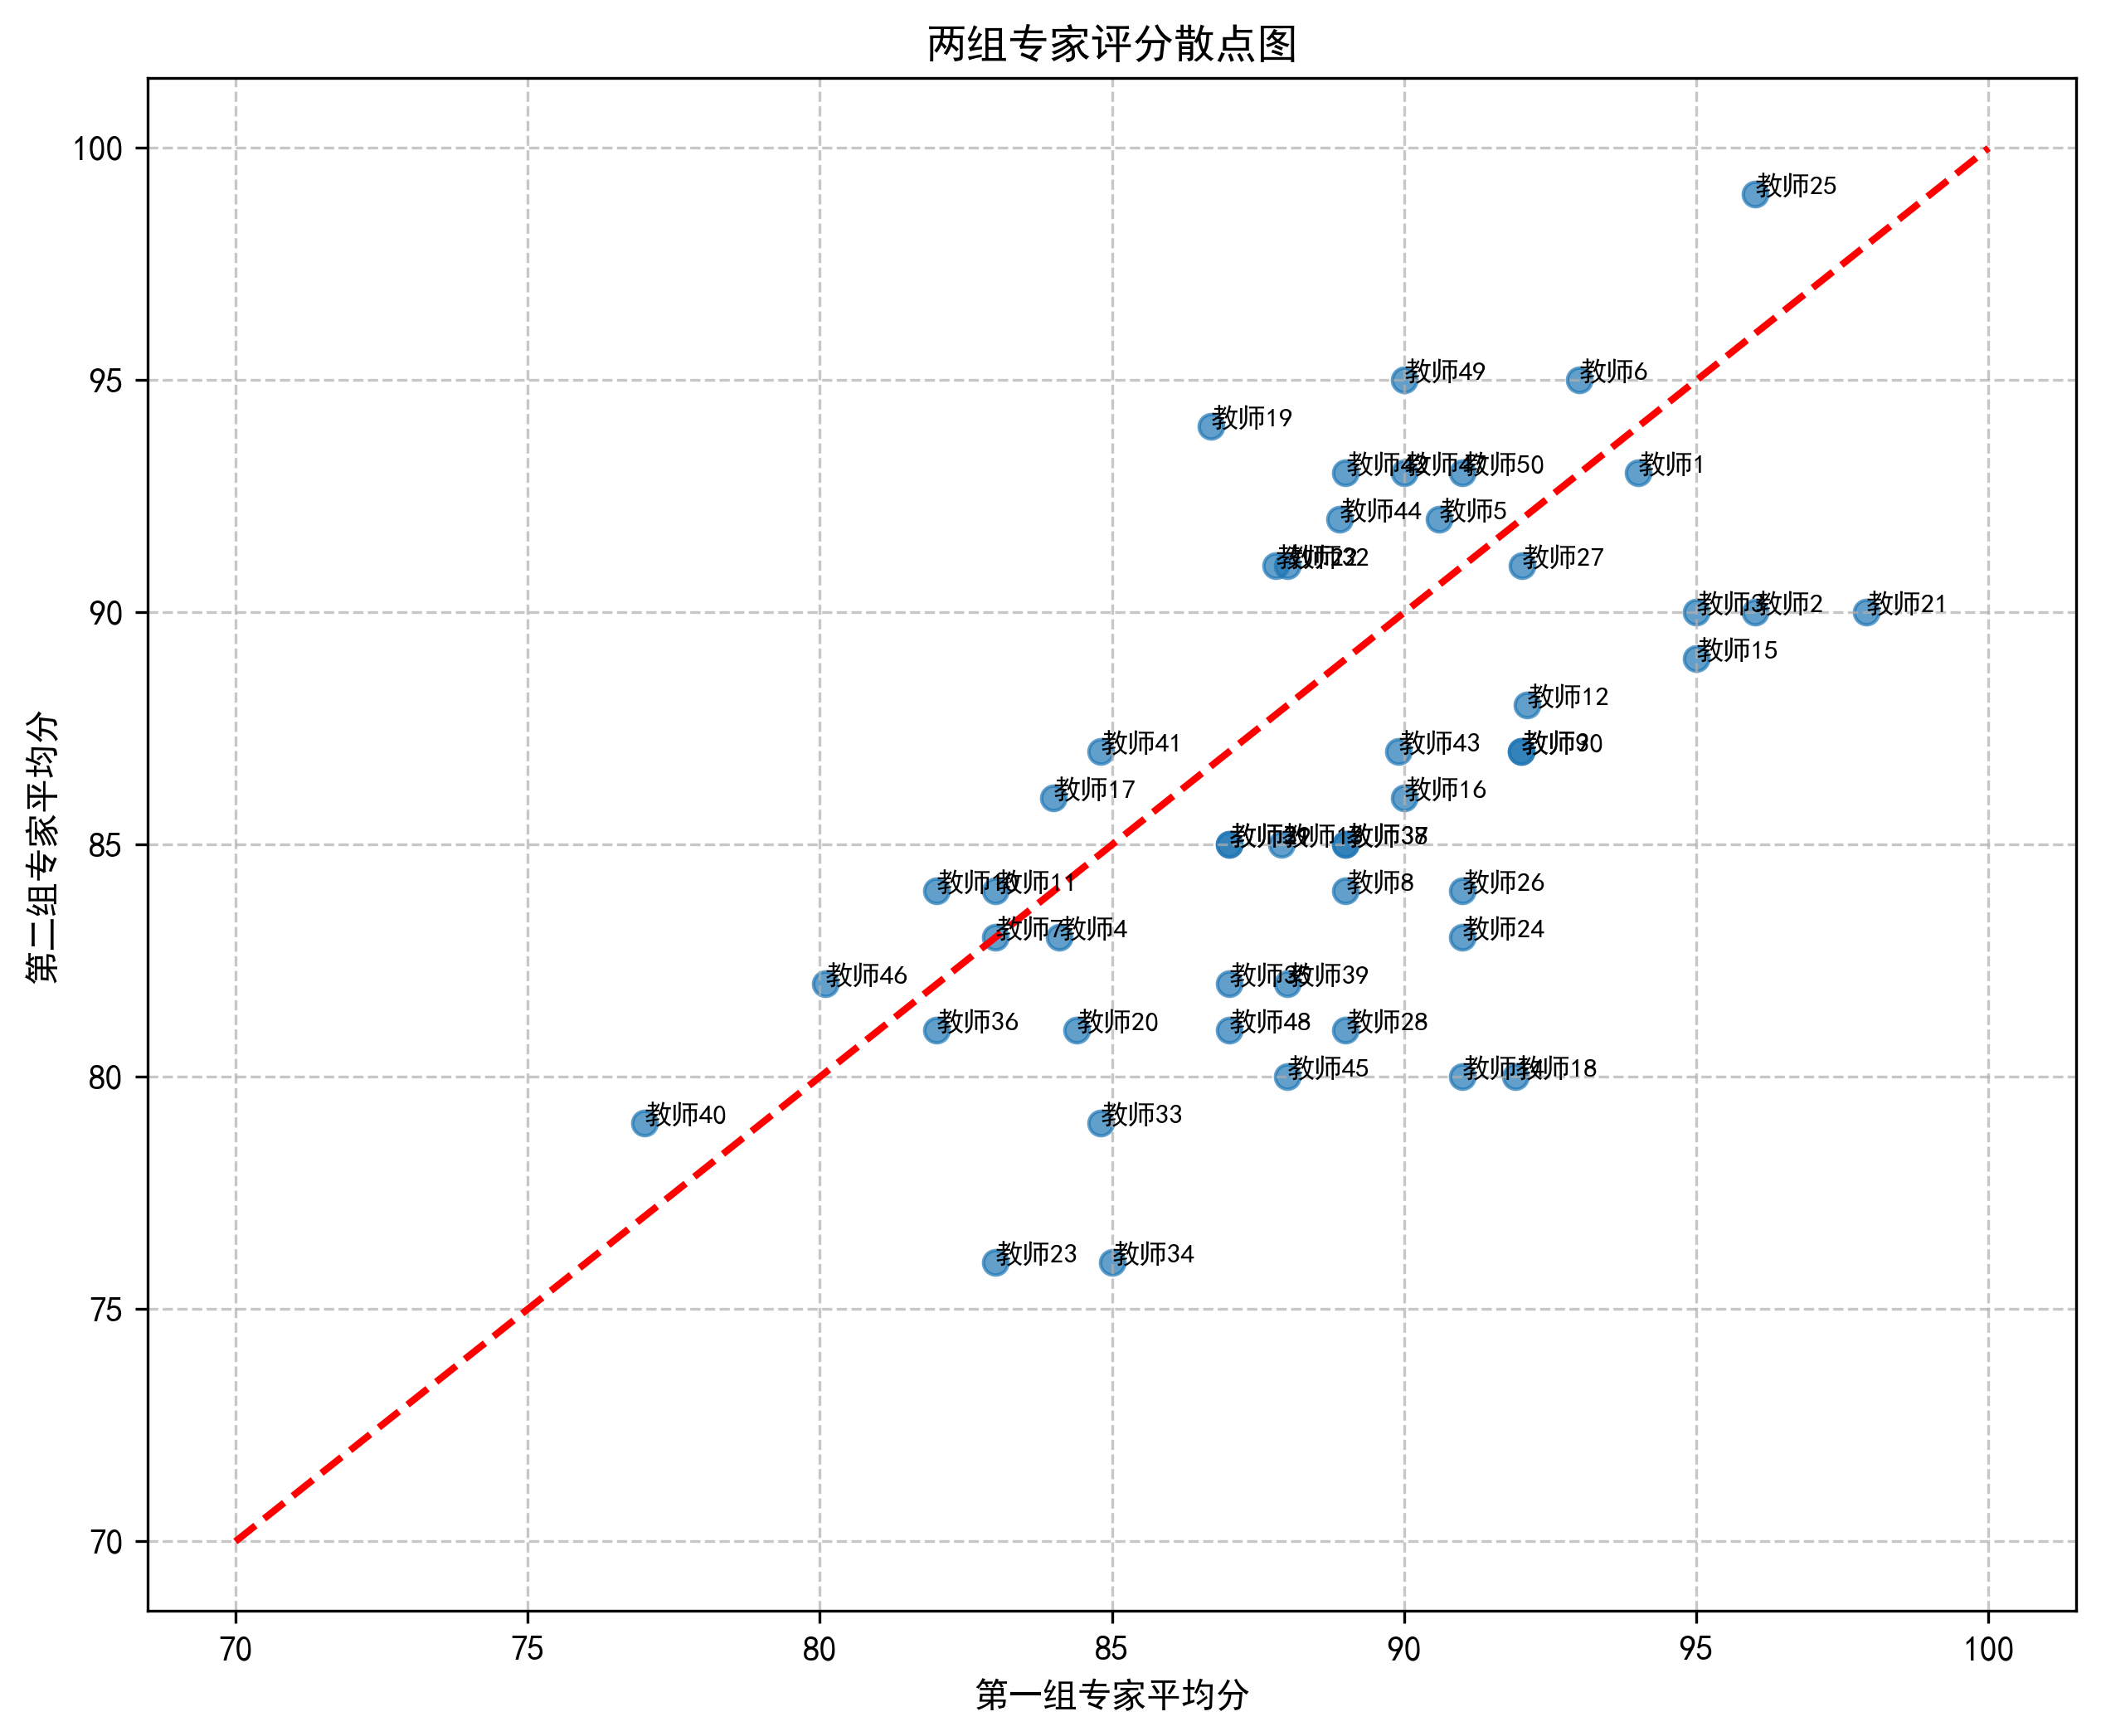
\includegraphics[width=0.6\textwidth]{scores_scatter.png} % 插入图片
    \caption{散点图}
\end{figure}


统计并对比两组评分的均值、标准差、极差、偏度、峰度等核心指标,并辅以箱线图、直方图等可视化手段直观展示分布形态、中心趋势、离散程度和潜在异常,为后续推断检验和一致性评估奠定基础。

\begin{figure}[htbp]
    \centering
    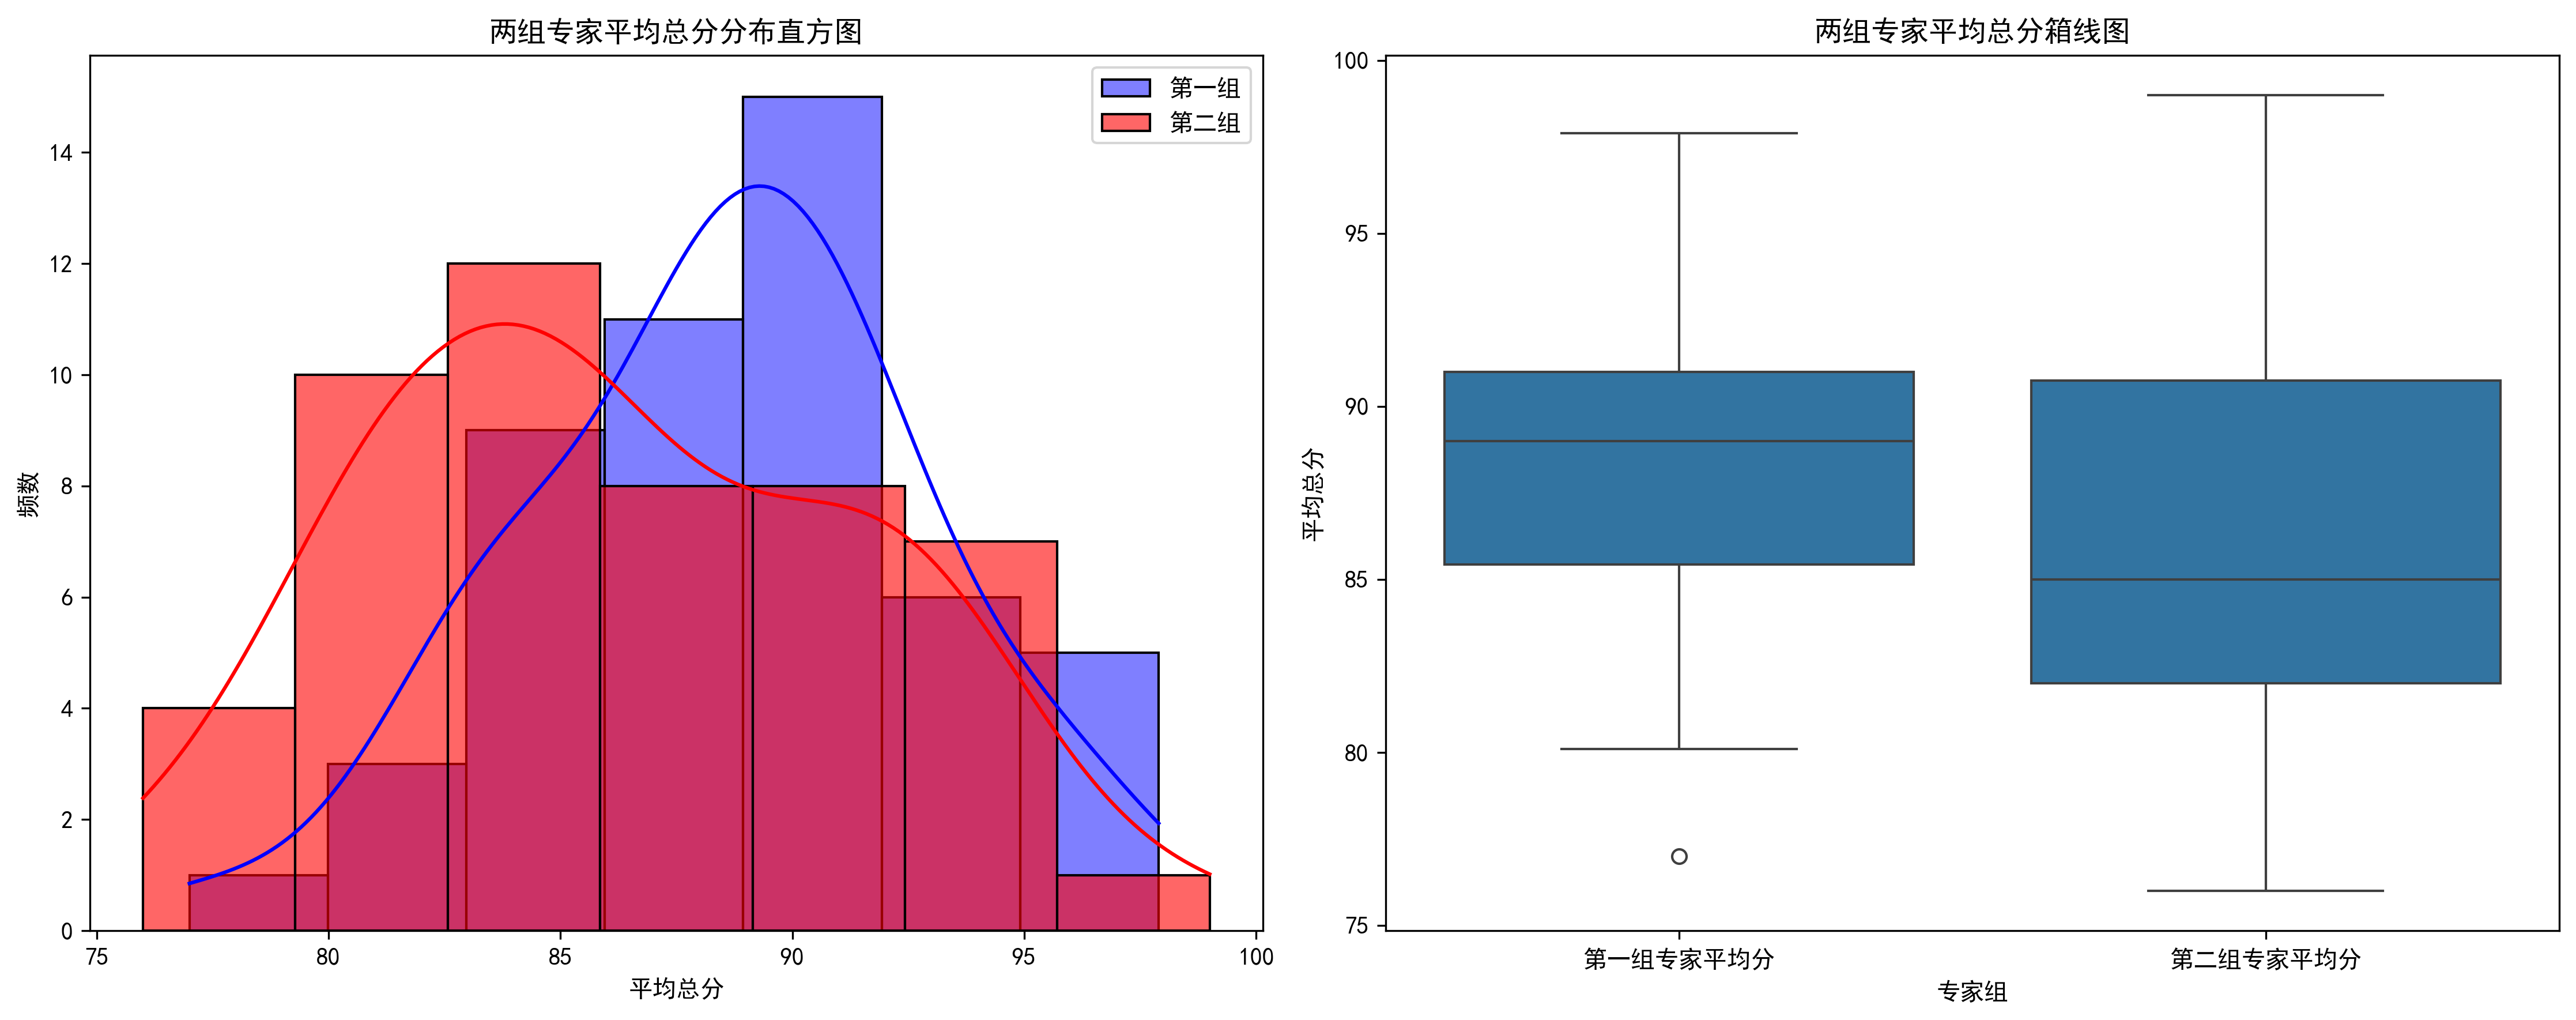
\includegraphics[width=1\textwidth]{descriptive_statistics.png} % 插入图片
    \caption{直方图和箱线图}
\end{figure}



对所有教师-专家数据,经清洗和缺失项均值填补后,分别求得两组专家每位教师的平均总分 $S^{(1)}_i, S^{(2)}_i$。以附件1为例,第一组专家评分均值88.54,标准差4.34,第二组均值86.18,标准差5.35,均略呈负偏态。表~\ref{tab:descstat} 总结描述性统计结果。



\begin{table}[h]
\centering
\caption{两组专家评分描述性统计}
\label{tab:descstat}
\begin{tabular}{lcc}
\toprule
统计指标 & 第一组专家评分 & 第二组专家评分 \\
\midrule
样本量      & 50        & 50        \\
均值        & 88.54     & 86.18     \\
标准差      & 4.34      & 5.35      \\
最小值      & 77.00     & 76.00     \\
极差        & 20.90     & 23.00     \\
偏度        & -0.23     & 0.23      \\
峰度        & -0.05     & -0.68     \\
\bottomrule
\end{tabular}
\end{table}

\subsection{显著性差异检验与效应量}
\subsubsection{配对显著性检验}
针对同一批教师的配对评分,先对两组评分差值$D_i$进行Shapiro-Wilk正态性检验。若近似正态,采用配对$t$检验对两组均值差异做统计推断;若非正态,则采用Wilcoxon符号秩检验。以$p$值小于0.05为统计显著,结合效应量判断实际意义。

\subsubsection{效应量量化}
采用配对样本下的Cohen's $d$量化两组专家均值差异的实际影响:
\[
d = \frac{\overline{D}}{s_D}
\]
其中$\overline{D}$为所有差值均值,$s_D$为样本标准差。$|d| \approx 0.2$为小效应,$\approx 0.5$为中等效应,$\approx 0.8$为大效应,这可弥补$p$值无法揭示实际影响大小的不足。

教师的两组专家平均分之差 $D_i = S^{(1)}_i - S^{(2)}_i$ 经Shapiro-Wilk检验$p=0.187$,近似正态,适合配对样本t检验。t检验$p=0.001$,两组专家评分存在统计学显著差异。Cohen's $d=0.52$,为中等效应,说明分组差异在实际教学评价中具备一定意义。

\subsection{专家组可靠性(内部一致性)分析}
采用组内相关系数ICC(Intraclass Correlation Coefficient)定量评价组内一致性。模型选用“双向随机效应、绝对一致性、单次测量”ICC(2,1)标准,是因为:

\begin{itemize}
    \item 双向随机效应假设专家和被评分教师均为总体的随机抽取,增强结论的普适性;
    \item 绝对一致性着重考察分数本身(非仅排名)的一致水平;
    \item 单次测量聚焦个别评分者一致性(适合专家组实际结构)。
\end{itemize}

ICC判据:$<0.5$为差;$0.5{\sim}0.75$为中等;$0.75{\sim}0.9$良好;$\geq0.9$优秀。

\begin{figure}[H]
    \centering
    \begin{minipage}[t]{0.5\textwidth}
        \centering
        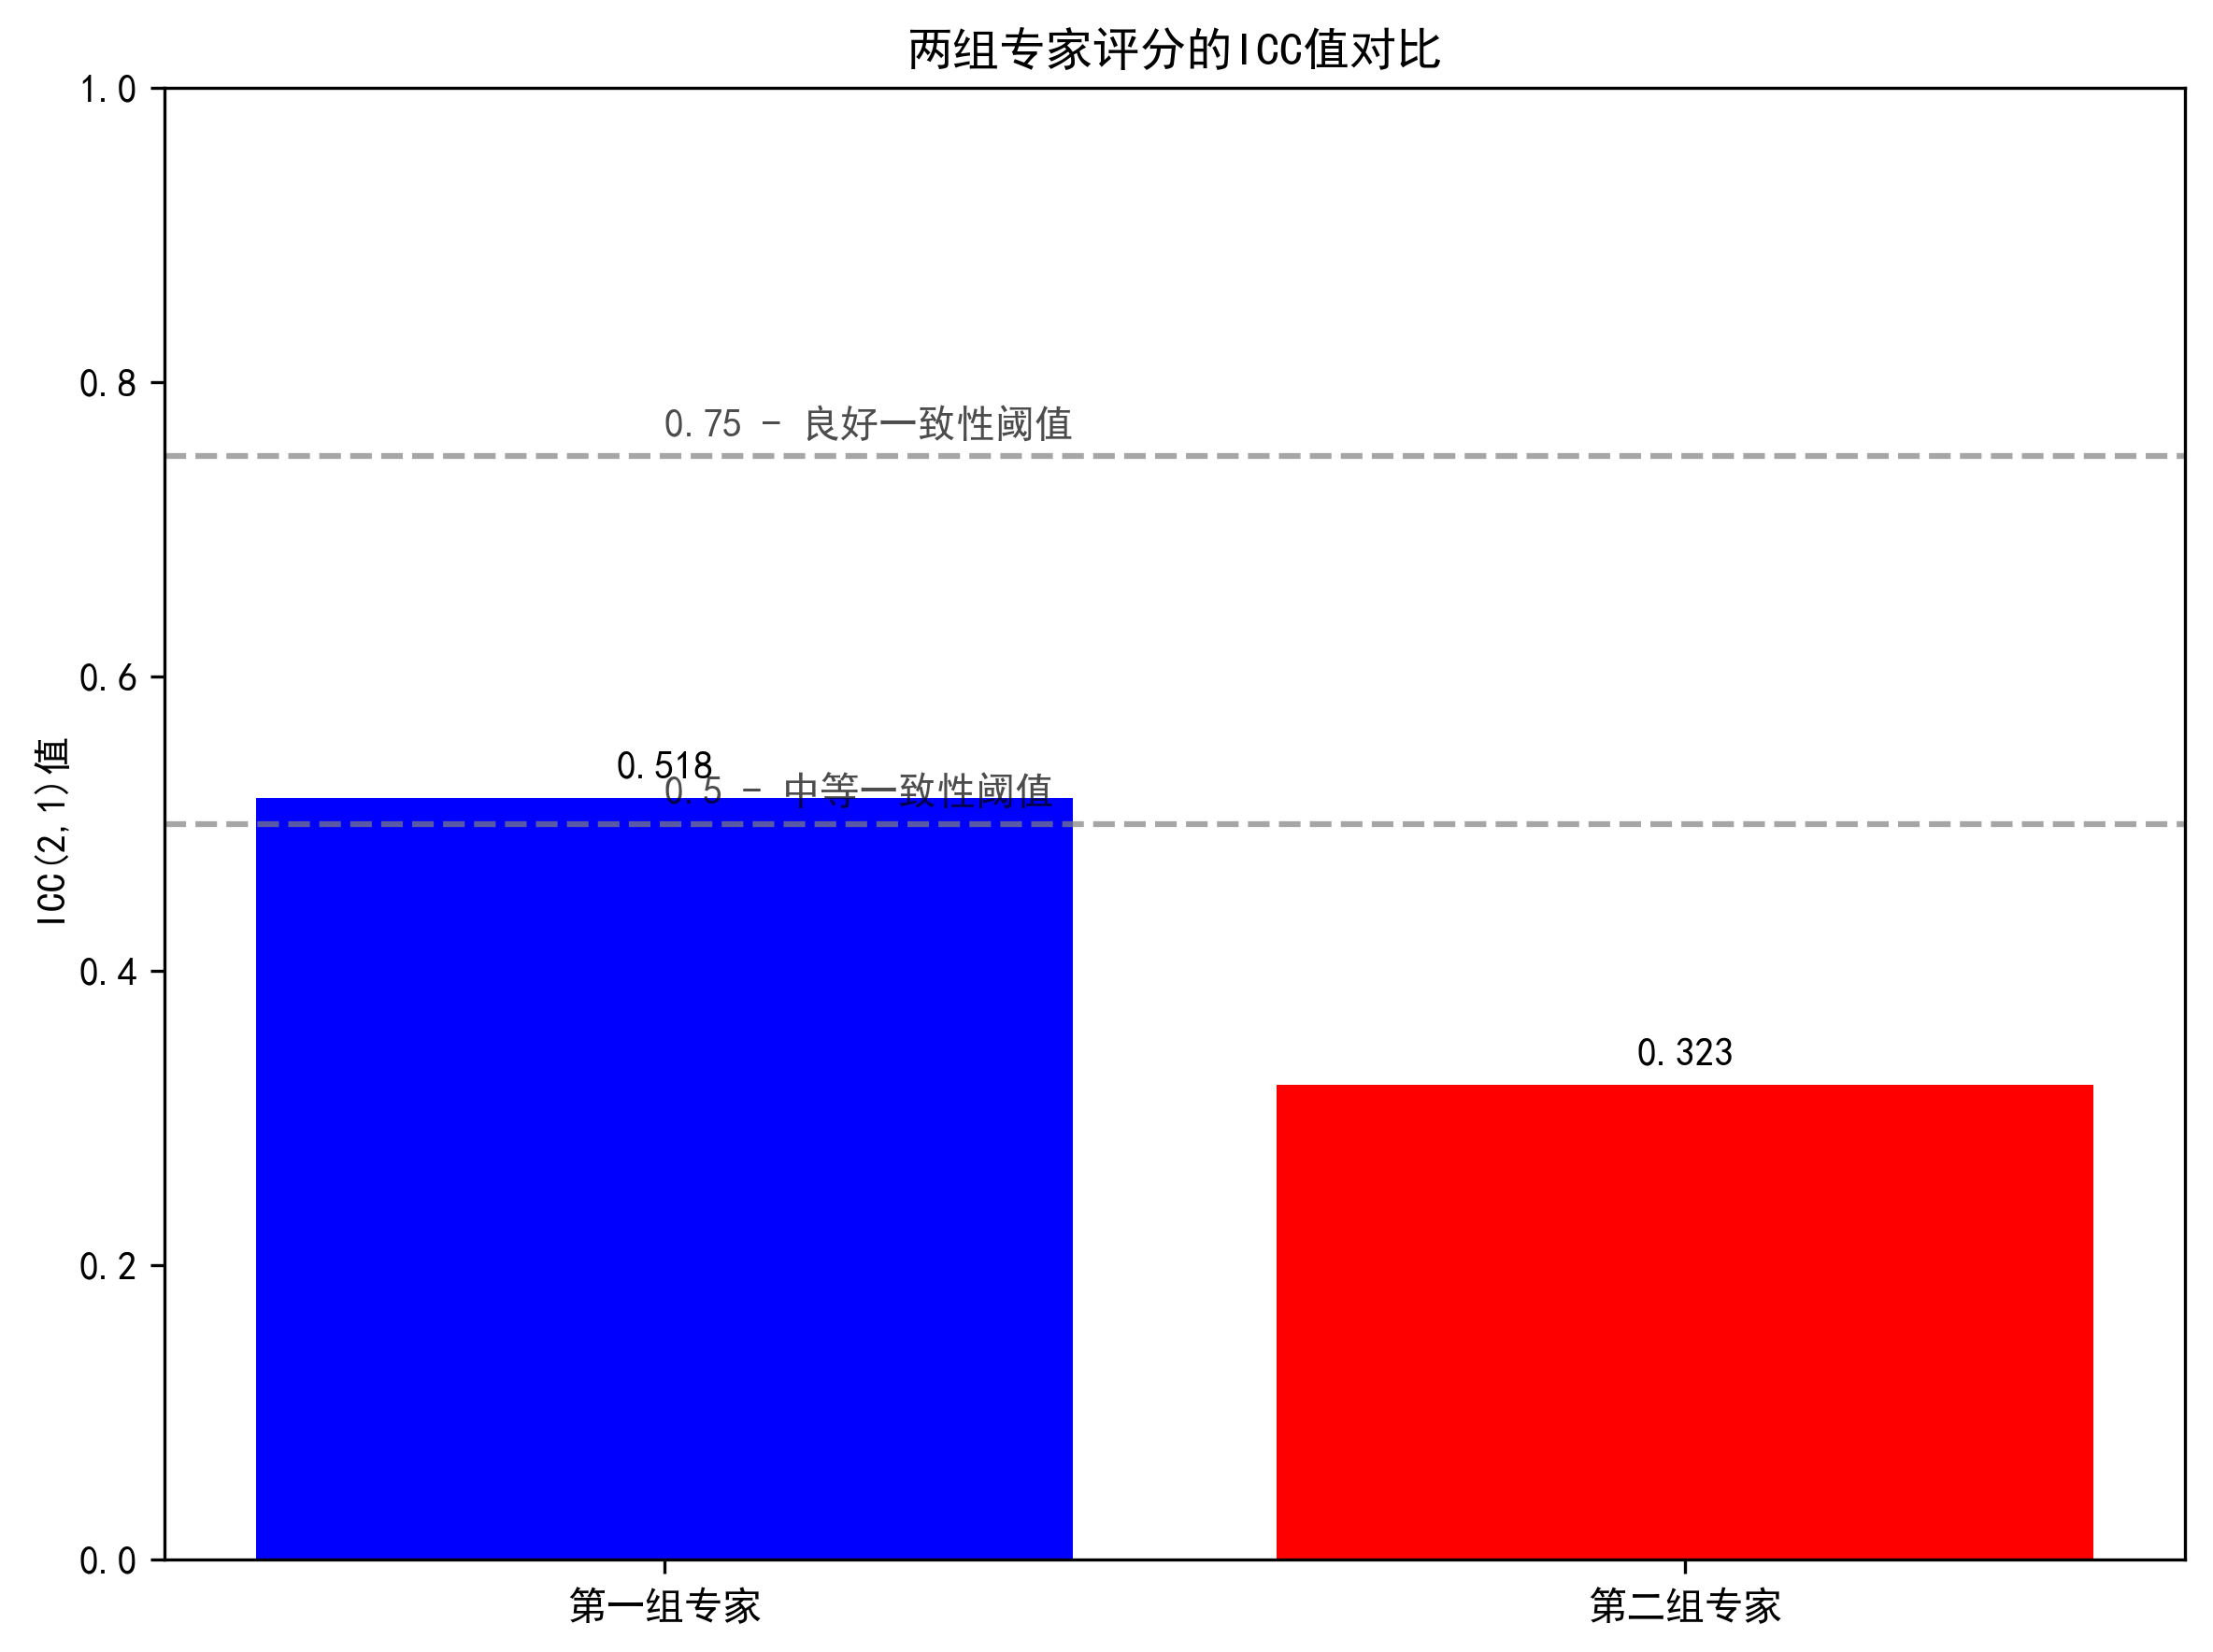
\includegraphics[width=1\textwidth]{icc_analysis.png}
    \end{minipage}
    \hfill
    \begin{minipage}[t]{1\textwidth}
        \centering
        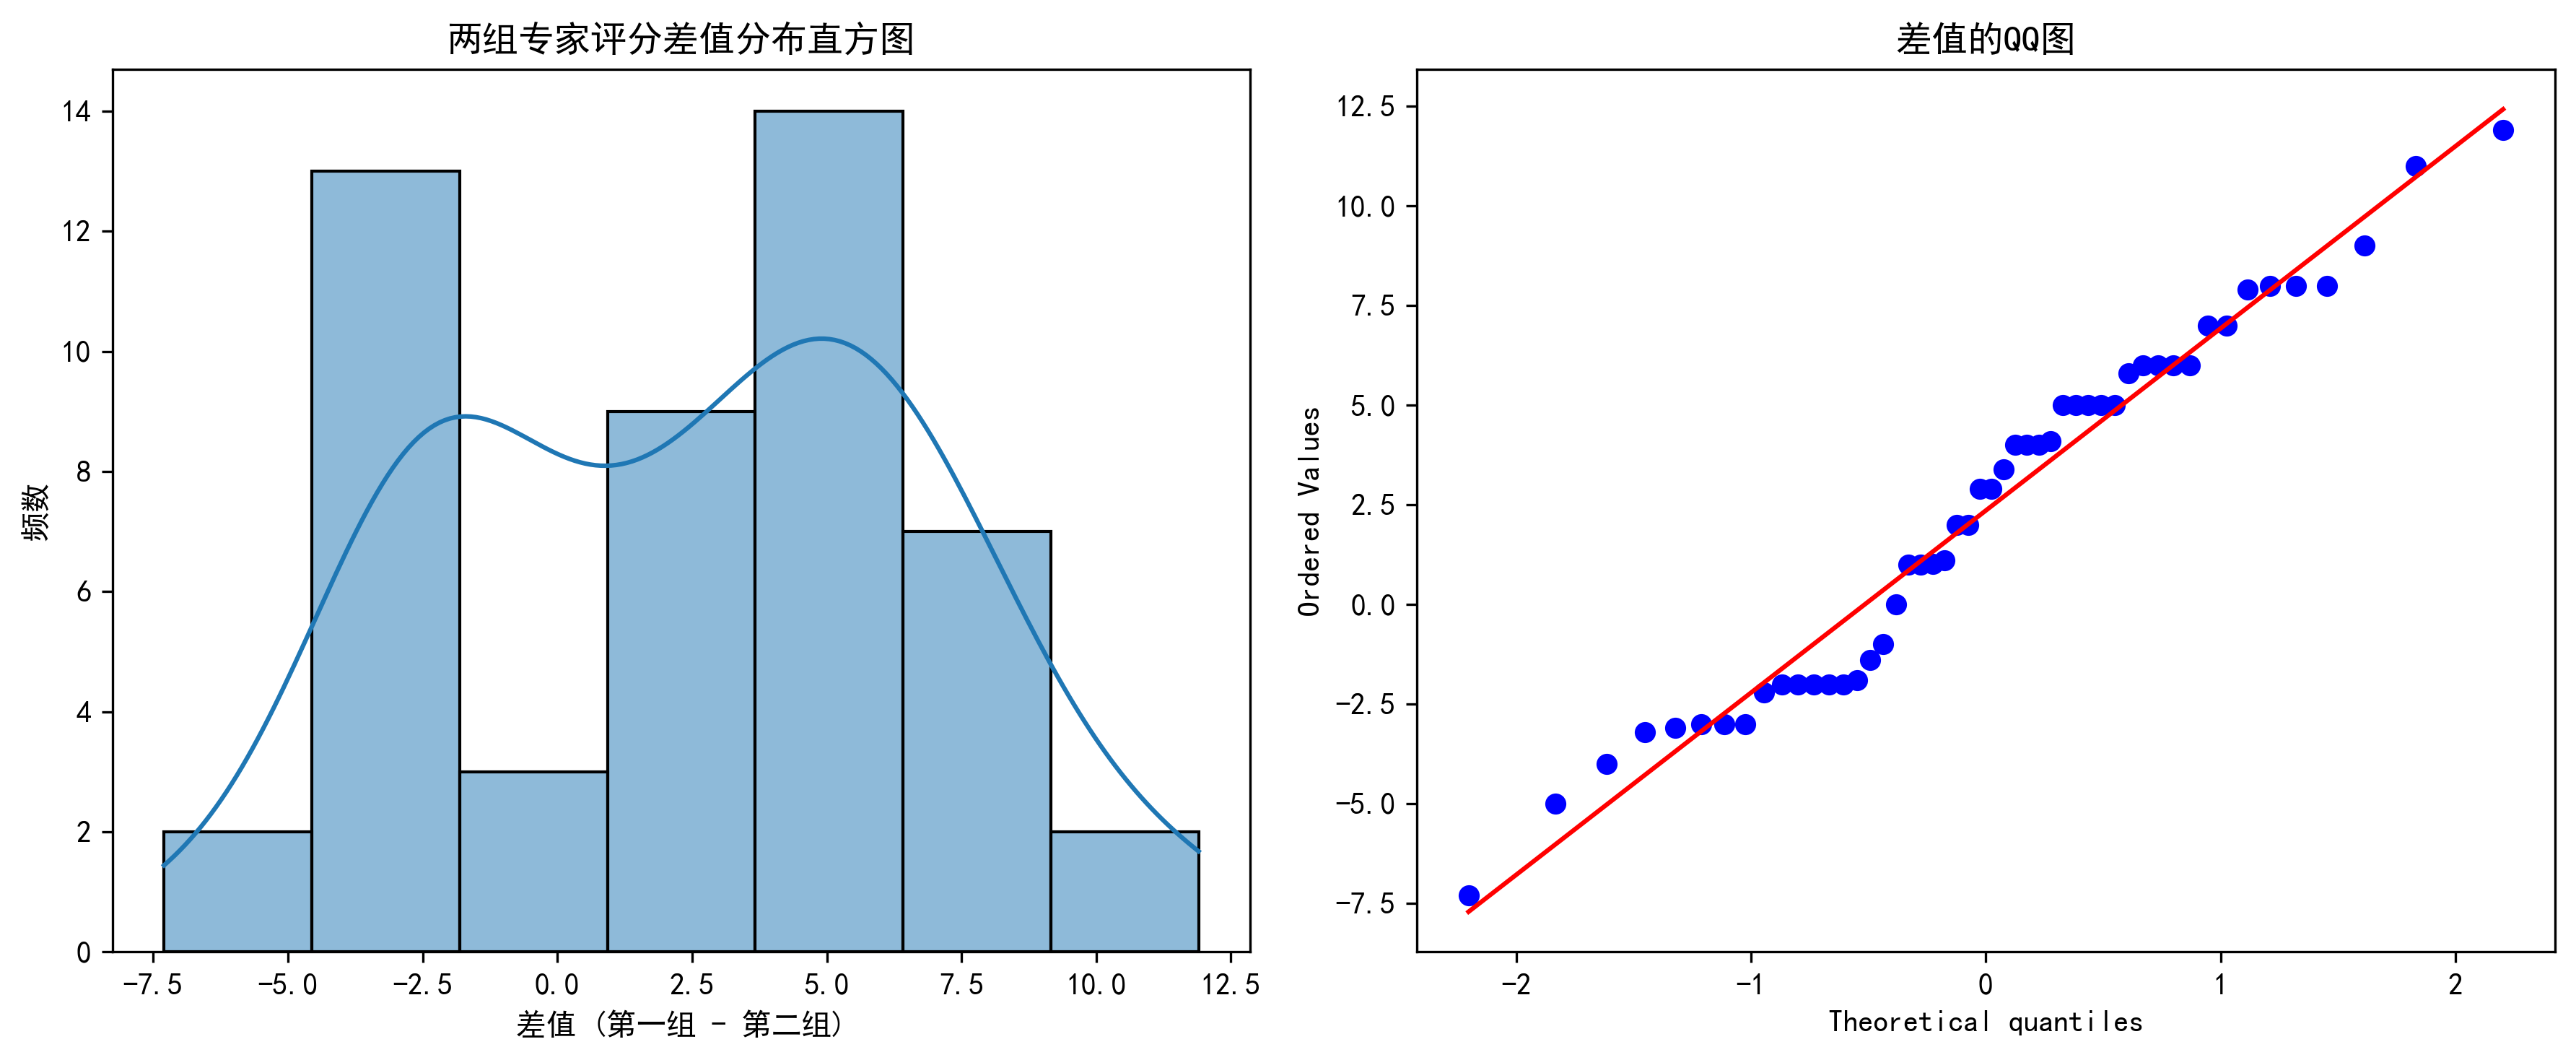
\includegraphics[width=1\textwidth]{normality_test.png}
    \end{minipage}
\end{figure}


分别计算两组专家内ICC(双向随机效应、绝对一致性、单次测量):
\begin{itemize}
    \item 第一组ICC=0.518(中等一致性)
    \item 第二组ICC=0.323(差/不可接受的一致性)
\end{itemize}
第一组专家在评分标准和评分稳定性方面表现更优,具有更高的一致性和集体信度。

\subsection{综合判断与结论}
以实际分析为例,经描述性统计,第一组均值高于第二组(88.54 vs 86.18),标准差更低。差值$D_i$正态性检验$p=0.187$,支持采用配对$t$检验,检验$p=0.001$,存在显著差异。Cohen's $d=0.522$,为中等效应。

ICC分析显示,第一组ICC=0.518(中等一致性),第二组ICC=0.323(偏低一致性)。表明第一组专家判分标准更统一、一致性更优,具备更高集体信度。

本节通过多层次分析证明,两组专家对同批教师的打分不仅分布中心存在统计显著差异($p=0.001$),而且差异效应为中等水平。同时,内部一致性检验结果显示,第一组专家的评分标准更统一,输出更稳定,因此结果更具可信度。建议在教师评价体系优化和赋分权重调整时,优先参考一致性更高的专家组评分。





\subsection{小结}
本文针对两组专家对同批教师的评分用配对t检验、效应量和ICC信度分析,科学评估了评分差异和组内一致性。研究流程严谨,既揭示了分组间差异的统计和实际意义,也为后续高校教学评价权威化、标准化提供了数据与思路支撑。





